\documentclass[a4paper,12pt]{scrartcl} % the percent sign is used for comments.
\usepackage[margin=3cm]{geometry} % sets the borders to 3cm each
\usepackage[english]{babel}     %defines language for spacing
\usepackage[T1]{fontenc}        % sets font to T1 and allows umlaute
\usepackage{lmodern}            % improves font display in PDFs
\usepackage{microtype}          % improves spacing when using lmodern
\usepackage{amsmath,amsfonts,amssymb}   % allows particular math environments
\usepackage{graphicx}           % allows using graphics
\usepackage{booktabs}           %allows creating professional tables with commands like \toprule
\usepackage{csquotes}           % better use of quotation marks, makes them context-sensitive
%\usepackage{longtable}          % allows for Table over more than one page
%\usepackage{sidewaystable}          % allows creating landscape tables
\usepackage[labelfont=bf,format=hang]{caption} % more powerful caption of figures and tables; The language for the caption label like Figure is boldface (bf). The language is taken from the babel package, i.e. Abbildung if german instead of english.

\usepackage{setspace}           % allows for \onehalfspacing and \doublespacing to set linespacing
\usepackage{epstopdf}           % allows using eps-file with pdflatex
\usepackage{textcomp}           % adds more symbols
%\usepackage{indentfirst}       % use if you want to indent first row
\usepackage{bigints} % for large integrals
\usepackage{dsfont} 
%%%% define the usage of BibLaTeX for citations and bibliographies
%\usepackage[%
%citestyle=authoryear-comp,%use compressed author-year citation
%bibstyle=JME,% use JME-style; change to JME_sentencecase to have all titles converted to lowercase letters
%maxbibnames=5,% %maximum number of names printed in bibliography before truncation with ``et al.'' is used
%minbibnames=1, % number of authors displayed if truncation happens
%maxnames=4,% maximum number of names printed in citation before et al. is used
%minnames=1,% number of authors displayed if truncation happens
%datezeros=false,% no leading 0 if dates are printed
%date=long,%
%isbn=false,% show no ISBNs
%natbib=true,% enable natbib-compatibility
%url=false,% show no urls
%backend=bibtex %use bibtex as backend
%]{biblatex}
%
%\addglobalbib{mybibfile.bib} % defines the name of the .bib-file	


\usepackage[pdfpagelabels=true,plainpages=false,pdftex,bookmarksnumbered=false,bookmarksopen=true]{hyperref}%plainpage and pdfpagelabels allows for correct figure links when using different page numberings
% bookmarksnumbered=false shuts off TOC numbers in TOC of PDF
% bookmarksopen=true opens TOC in Abobe Reader on the left


\hypersetup{
pdfproducer = {LaTeX},
colorlinks,
linkcolor=black,
filecolor=yellow,
urlcolor=blue,
citecolor=black,
pdftitle ={Title of the thesis},
pdfsubject ={Thesis},
pdfauthor = {Your Name },
pdfkeywords = {Some keywords}
pdfcreator={pdfLaTex}}


\usepackage[%
nonumberlist, %switch of displaying page numbers
acronym,      %creates List of Abbreviations
%toc,          %triggers entry into table of content
%section      %defines the level where the TOC entry appears
]{glossaries} % used to create list of symbols and abbreviations; one of the few packages to be defined after hyperref

\newglossary[slg]{symbolslist}{syi}{syg}{List of Symbols} %defines a new list called symbolslist for the List of symbols

\makeglossaries %need for sorting of entries to list of symbols and abbreviations; must be defined after all \newglossary commands

%% define terms for List of Symbols; entries only appear if they have been referenced in the main document  using either \gls{} or \glsadd{}

\newglossaryentry{symb:pi}{%
    name={\ensuremath{\pi}}, %define symbol; the \ensuremath ensures the symbol can be used inside and outside math environments
    description={ratio of circumference of circle to its diameter}, % the description that appears in the list of symbols
    sort=symbolpi, % key for sorting the symbols
    type=symbolslist % specifies that the entry belongs to the symbolslist-list and not the default (acronym) list
    }

\newglossaryentry{symb:i}{name={\ensuremath{i}},description={square root of $-1$},sort=symboli,type=symbolslist}
\newglossaryentry{symb:e}{name={\ensuremath{e}},description={Euler number},sort=symbole,type=symbolslist}

\newacronym{acro:OLS}{OLS}{Ordinary Least Squares}%defines the acronym OLS
\glsadd{acro:OLS} % add the acronym to the list of abbreviations, regardless of whether it has been used in the document

\onehalfspacing

% ________________ Set up the document ______________________%

\pagestyle{plain}          % empty header, page number in the middle of the footer

\setcounter{tocdepth}{3}   % The Table of contents is three levels deep, i.e. down to subsubsections.

% ________________ Set up new commands ______________________%
\newcommand{\nin}{\not\in}
\newcommand{\bs}{\boldsymbol}  % shortcut to generate bold symbols in math environments
\newcommand{\pt}{\propto}

\newcommand{\sumd}{\sum_{d=1}^D}
\newcommand{\sumt}{\sum_{t=1}^T}
\newcommand{\sumiN}{\sum_{i=1}^N}
\newcommand{\sumaM}{\sum_{m_a=1}^M}
\newcommand{\sumbM}{\sum_{m_b=1}^M}
\newcommand{\sumpM}{\sum_{m_p=1}^M}
\newcommand{\sumqM}{\sum_{m_q=1}^M}
\newcommand{\sumJd}{\sum_{j=1}^{J_d}}

\newcommand{\prodd}{\prod_{d=1}^D}
\newcommand{\prodt}{\prod_{t=1}^T}
\newcommand{\prodn}{\prod_{n=1}^{N}}
\newcommand{\prodJ}[1]{\prod_{j=1}^{J_{#1}}}







% ________________ Defines command \ScaleIfNeeded that scales Figures to width of the page if they are larger ______________________%

\makeatletter
\def\ScaleIfNeeded{%
\ifdim\Gin@nat@width>\linewidth
\linewidth
\else
\Gin@nat@width
\fi
}
\makeatother


\begin{document}

% ________________ Title Page ______________________%



\pagenumbering{roman}   % Roman numbering

\begin{titlepage}

\thispagestyle{empty}   % no number on titlepage
%%%% to be deleted, only for information purposes
%%%%%


\begin{center}
\vspace*{2.cm}
{\textbf{\large{Simultaneous Bayesian Modelling of a Panel of
Parametric Income Distributions for Grouped Data}}} \\
\vspace*{2cm}
Bastian Gribisch \& Ilya Zarubin\\
%\vspace{0.5cm}
%Department of Economics\\
%University of Mannheim\\
%\vspace*{0.5cm}
%submitted to:\\
%Prof. Dr. Johannes Pfeifer\\
%\vspace*{0.5cm}

\end{center}


\vfill
\begin{flushright}
   \emph{submitted by:} \\
   \emph{Ilya Zarubin} \\
   \vspace*{0.5cm}
   \emph{zarubin@wiso.uni-koeln.de}\\
\end{flushright}


\end{titlepage}

\clearpage                % forces a new page and setting of current float objects stored by Latex



% ________________ Table of Contents/Figures/Tables ______________________%

%\tableofcontents
\clearpage
%\listoffigures
\clearpage
%\listoftables
%\clearpage
%\printglossary[type=\acronymtype,style=long,title=List of Abbreviations]
%\clearpage
%\printglossary[type=symbolslist,style=long,title=List of Symbols]
%\clearpage

% ________________ Main Matter ______________________%

\pagenumbering{arabic}      % Arabic Numbering
\setcounter{page}{1}        % Start Numbering at 1


\section{Model I}
\subsection*{Assumptions}
\begin{itemize}
\item for a fixed cross sectional unit $i$ at some time point $t$:\\ $\bs{\bar{n}}_{it}=\left(n_{it}^{(1)},\ldots,n_{it}^{(M_{it})}\right)$: number of observations in the $M_{it}$ income groups 
\item we consider a panel of observations where the number of income groups may vary over both indices but typically changes only with $i$ i.e. $M_{it}\equiv M_{i}$
\item[\underline{\textbf{\textit{Assumption 1:}}}] let each $\bs{\bar{n}}_{it}\overset{ind.}{\sim} \text{MNL}_{it}\left(\pi_{it}^{(1)},\ldots,\pi_{it}^{(M_{it})}\right)$ conditional on regressors $x_{it}$\\
hence the joint likelihood function is
\begin{align*}
L\left(\left\{\theta_{it}\right\};\left\{\bs{\bar{n}}_{it}\right\}\right)=\prod_{i=1}^N \prod_{t=1}^T \text{MNL}_{it}(\pi_{it}^{(1)},\ldots,\pi_{it}^{(M_{it})})\;,
\end{align*}
where each $\pi_{it}^{(k)}=\left(F_y(z_{it}^{(k)};\theta_{it})-F_y(z_{it}^{(k-1)};\theta_{it})\right)$ and some parametric income distribution $F_y(y;\theta)$ with $P$-variate parameter vector  $\theta=(\theta^{(1)},\ldots,\theta^{(P)})$.
\item key point of distributional regression: link each parameter component $\theta^{(p)}_{it}$ to a \textit{structured additive predictor} $\eta_{it}^{(p)}$ via a response function $h_{(p)}$
\begin{align*}
\theta_{it}^{(p)} = h_{p}(\eta_{it}^{(p)})\;,
\end{align*}
where $h^{(p)}$'s range equals $\theta_{it}^{(p)}$'s possible parameter values e.g. $\exp(\cdot)$ for $\theta_{it}^{(p)}>0$ \\
The predictor specification allows each $\theta_{it}^{(p)}$ to  depend on $J_p$ different effects e.g. linear or random effects denoted as $x_{(it)}$'s or $u_i$,  respectively
\begin{align*}
\eta_{it}^{(p)}=x_{(it,1)}^{\prime}\beta_1^{(p)}+
\ldots+x_{(it,J_p)}^{\prime}
\beta_{J_p}^{(p)}+u_i^{(p)}\;,
\end{align*}
\item Number of parameters: $J_1 \times J_2\times\ldots \times J_P$ different (multivariate) $\beta$'s and $N\times P$ different random effects $u_i$.
\item[\underline{\textbf{\textit{Assumption 2:}}}] To specify an  income distribution function we assume a rather general four-parameter GB2:
\begin{align*}
F(y;a,b,p,q)=B(d;p,q)=\frac{\int_{0}^d t^{p-1}(1-t)^{q-1}dt}{\text{B}(p,q)}\;,~d=\frac{(y/b)^a}{1+(y/b)^a}\;,
\end{align*}
where each parameter is strictly positive  $a,b,p,q>0$
%
%
%
%
%
\clearpage
%
%
%
%
%
\item Hence, in a panel setting the parameters are  $a_{it}=\theta_{it}^{(1)}$, $b_{it}=\theta_{it}^{(2)}$, $p_{it}=\theta_{it}^{(3)}$, $q_{it}=\theta_{it}^{(4)};,$ and all are equipped with strictly positive response function $\forall i,t:$ 
\begin{align*}
a_{it}&=h\left(\eta_{it}^{(a)}\right)=
\exp\left(\eta_{it}^{(a)}\right)\;,~~~b_{it}=h\left(\eta_{it}^{(b)}\right)=
\exp\left(\eta_{it}^{(b)}\right)\;,\\
p_{it}&=h\left(\eta_{it}^{(p)}\right)=
\exp\left(\eta_{it}^{(p)}\right)\;,~~~q_{it}=h\left(\eta_{it}^{(q)}\right)=
\exp\left(\eta_{it}^{(q)}\right)\;,
\end{align*}
and corresponding additive predictors
\begin{align*}
\eta_{it}^{(a)}&=\left(x_{it}^{(a)}\right)^{\prime}\beta^{(a)} + u_i^{(a)}\;,~~~
\eta_{it}^{(b)}=\left(x_{it}^{(b)}\right)^{\prime}\beta^{(b)} + u_i^{(b)}\;,~~~\\
\eta_{it}^{(p)}&=\left(x_{it}^{(p)}\right)^{\prime}\beta^{(p)} + u_i^{(p)}\;,~~~
\eta_{it}^{(q)}=\left(x_{it}^{(q)}\right)^{\prime}\beta^{(q)} + u_i^{(q)}\;,
\end{align*}
where the $\beta$'s may be multivariate and $u_i$'s are random effects.
\end{itemize}
\subsection*{Bayesian model formulation:}
We follow Klein \textit{et al.} (2013) and consider a Bayesian setting:
\begin{align*}
p\left(\boldsymbol{\beta},\boldsymbol{U},\boldsymbol{\sigma},\boldsymbol{\tau}|\bar{\boldsymbol{N}},\boldsymbol{X}\right)
\propto p\left(\bar{\boldsymbol{N}}|\boldsymbol{\beta},\boldsymbol{U},\boldsymbol{X}\right)p\left(\boldsymbol{\beta}|\boldsymbol{\tau}\right)p\left(\boldsymbol{\tau}\right)
p\left(\boldsymbol{U}|\boldsymbol{\sigma}\right)p(\boldsymbol{\sigma})\;,
\end{align*}
where the components are
\begin{itemize}
\item deterministic regressors 
$
\boldsymbol{X}=
\left(\boldsymbol{x}_{it}\right)_{i,t}^{N,T}=
\left(
x_{it}^{(a)},x_{it}^{(b)},x_{it}^{(p)},x_{it}^{(q)}
\right)_{i,t}^{N,T}
$ 
\item the (multivariate) panel data  
$
\bar{\boldsymbol{N}}=
\left(\boldsymbol{\bar{n}}_{it}\right)_{i,t}^{N,T}=
\left(n_{it}^{(1)},\ldots,n_{it}^{(M_{it})}\right)_{i,t}^{N,T}$ 
\item the (multivariate) parameters 
$\boldsymbol{\beta}=
\left(
\boldsymbol{\beta}_{a},\boldsymbol{\beta}_{b},
\boldsymbol{\beta}_{p},\boldsymbol{\beta}_{q}
\right)
$
\item beta prior variances
$\boldsymbol{\tau}=
\left(
\tau_{a},\tau_{b},\tau_{p},\tau_{q}
\right)
$
\item and random effects $\boldsymbol{U}=\left(\boldsymbol{U}_i\right)_{i=1}^N=\left(u_i^{(a)},u_i^{(b)},u_i^{(p)},u_i^{(q)}\right)_{i=1}^N$
\item random effect prior variances
$\boldsymbol{\sigma}=
\left(
\sigma_{a},\sigma_{b},\sigma_{p},\sigma_{q}
\right)
$
\end{itemize}
and where the corresponding prior and likelihood specifications are
\begin{itemize}
\item $p\left(\boldsymbol{\beta}|\tau\right)=
p\left(\boldsymbol{\beta_a}|\tau_{a}\right)
p\left(\boldsymbol{\beta_b}|\tau_{b}\right)
p\left(\boldsymbol{\beta_p}|\tau_{p}\right)
p\left(\boldsymbol{\beta_q}|\tau_{q}\right)$,
with each $\boldsymbol{\beta}|\tau\sim N(0,\tau^2)$
\item $p\left(\bs{U}\right)=\prod_{i=1}^N p(\boldsymbol{U}_i|\boldsymbol{\sigma})$ and $p(\boldsymbol{U}_i|\boldsymbol{\sigma})=
p\left(u_i^{(a)}|\sigma_{a}\right)
p\left(u_i^{(b)}|\sigma_{b}\right)
p\left(u_i^{(p)}|\sigma_{p}\right)
p\left(u_i^{(q)}|\sigma_{q}\right)
$,
with each $u_i|\sigma\sim N(0,\sigma^2)$ 
\item 
$
p
\left(
\bar{\boldsymbol{N}}|
\boldsymbol{\beta},\boldsymbol{U},
\boldsymbol{X}
\right)=
\prod_{i=1}^N \prod_{t=1}^T \text{MNL}_{it}\left(\pi_{it}^{(1)},\ldots,\pi_{it}^{(M_{it})}\right)$ 
is the joint multinom. likelihood, $\pi_{it}^{(k)}=\left(F_{\text{GB2}}
(z_{it}^{(k)};a_{it},b_{it},p_{it},q_{it})-F_{\text{GB2}}(z_{it}^{(k-1)};a_{it},b_{it},p_{it},q_{it})\right)$
\end{itemize}
\clearpage
\section{Estimation}
\subsection{MAP estimation (maximization w.r.t. posterior kernel)}
\subsubsection{Including maximization over RE}
\begin{align*}
\Theta_{\text{MAP}}
&= \underset{\boldsymbol{\beta},\boldsymbol{U},\boldsymbol{\sigma},\boldsymbol{\tau}}{\arg\max \;}
p\left(\boldsymbol{\beta},\boldsymbol{U},\boldsymbol{\sigma},\boldsymbol{\tau}|\bar{\boldsymbol{N}},\boldsymbol{X}\right)\\
&= \underset{\boldsymbol{\beta},\boldsymbol{U},\boldsymbol{\sigma},\boldsymbol{\tau}}{\arg\max \;}
p\left(\bar{\boldsymbol{N}}|\boldsymbol{\beta},\boldsymbol{U},\boldsymbol{X}\right)
\times p\left(\boldsymbol{\beta}|\boldsymbol{\tau}\right)\times p(\boldsymbol{\tau})
\times p\left(\boldsymbol{U}|\boldsymbol{\sigma}\right)\times p(\boldsymbol{\sigma})\\
&= \underset{\boldsymbol{\beta},\boldsymbol{U},\boldsymbol{\sigma},\boldsymbol{\tau}}{\arg\max \;}
\prod_{i=1}^N \prod_{t=1}^T \text{MNL}_{it}\left(\pi_{it}^{(1)},\ldots,\pi_{it}^{(M_{it})}\right)\\
&\times 
p\left(\boldsymbol{\beta_a}|\tau_a\right)
p\left(\boldsymbol{\beta_b}|\tau_b\right)
p\left(\boldsymbol{\beta_p}|\tau_p\right)
p\left(\boldsymbol{\beta_q}|\tau_q\right)
\times p(\tau_a)p(\tau_b)p(\tau_p)p(\tau_q)
\\
&\times \prod_{i=1}^N
p\left(u_i^{(a)}|\sigma_{a}\right)p\left(u_i^{(b)}|\sigma_{b}\right)p\left(u_i^{(p)}|\sigma_{p}\right)p\left(u_i^{(q)}|\sigma_{q}\right)
\times p(\sigma_a)p(\sigma_b)p(\sigma_p)p(\sigma_q)\;.
\end{align*}
\subsubsection{Without RE}
Integrating out all random effects $u_i^{(a)},u_i^{(b)},u_i^{(p)},u_i^{(q)}$ leads
\begin{align*}
\int_{\mathcal{U}}p\left(\boldsymbol{\beta},\boldsymbol{U},\boldsymbol{\sigma},\boldsymbol{\tau}|\bar{\boldsymbol{N}},\boldsymbol{X}\right)d\boldsymbol{U}
&=
\int_{\mathcal{U}}
p\left(\bar{\boldsymbol{N}}|\boldsymbol{\beta},\boldsymbol{U},\boldsymbol{X}\right)
p\left(\boldsymbol{U}|\boldsymbol{\sigma}\right)d\boldsymbol{U}\; \times 
p(\boldsymbol{\sigma})p\left(\boldsymbol{\beta}|\boldsymbol{\tau}\right)p(\boldsymbol{\tau})
p(\boldsymbol{\sigma})\;,
\end{align*}
with product space $\mathcal{U}=\times_{i=1}^N \mathcal{U}_i^{\mathcal{A}\times \mathcal{B}\times \mathcal{P}\times \mathcal{Q}}$ and  $\boldsymbol{U}_i=\left(u_i^{(1)},u_i^{(2)},
u_i^{(3)},u_i^{(4)}\right)$ living in $ \mathcal{U}_i^{\mathcal{A}\times \mathcal{B}\times \mathcal{P}\times \mathcal{Q}}$.
Hence, the MAP estimator for the structural parameters $\Theta_{\text{MAP}}^{\textbf{S}}$ only is
\begin{align*}
\Theta_{\text{MAP}}^{\textbf{S}}
&=
\underset{\boldsymbol{\beta},\boldsymbol{\sigma},\boldsymbol{\tau}}{\arg\max \;}
p\left(\boldsymbol{\beta},\boldsymbol{\sigma},\boldsymbol{\tau}|\bar{\boldsymbol{N}},\boldsymbol{X}\right)\\
&=
\underset{\boldsymbol{\beta},\boldsymbol{\sigma},\boldsymbol{\tau}}{\arg\max \;}
\int_{\mathcal{U}}
p\left(\boldsymbol{\beta},\boldsymbol{U},\boldsymbol{\sigma},\boldsymbol{\tau}|\bar{\boldsymbol{N}},\boldsymbol{X}\right)d\boldsymbol{U} \\
&=
\underset{\boldsymbol{\beta},\boldsymbol{\sigma},\boldsymbol{\tau}}{\arg\max \;}
\int_{\mathcal{U}}
p\left(\bar{\boldsymbol{N}}|\boldsymbol{\beta},\boldsymbol{U},\boldsymbol{X}\right)
p\left(\boldsymbol{U}|\boldsymbol{\sigma}\right)d\boldsymbol{U}
\times
p(\boldsymbol{\sigma})p\left(\boldsymbol{\beta}|\boldsymbol{\tau}\right)p(\boldsymbol{\tau})\;\\
&=
\underset{\boldsymbol{\beta},\boldsymbol{\sigma},\boldsymbol{\tau}}{\arg\max \;}
\prod_{i=1}^N 
\int_{\mathcal{U}_i^{\mathcal{A}\times \mathcal{B}\times \mathcal{P}\times \mathcal{Q}}} 
\prod_{t=1}^T
\text{MNL}_{it}\left(\pi_{it}^{(1)},\ldots,\pi_{it}^{(M_{it})}\right)
p\left(\boldsymbol{U}_i|\boldsymbol{\sigma}\right)d\boldsymbol{U}_i\\
&\times
p(\boldsymbol{\sigma})p\left(\boldsymbol{\beta}|\boldsymbol{\tau}\right)p(\boldsymbol{\tau})\;,
\end{align*}
The integral to be approximated via quadrature (i.e. to be evaluated numerically) is
\begin{align*}
\mathcal{I}_{RE}&=\int_{\mathcal{U}_i^{\mathcal{A}\times \mathcal{B}\times \mathcal{P}\times \mathcal{Q}}} 
\prod_{t=1}^T
\text{MNL}_{it}\left(\pi_{it}^{(1)},\ldots,\pi_{it}^{(M_{it})}\right)
p\left(\boldsymbol{U}_i|\boldsymbol{\sigma}\right)d\boldsymbol{U}_i\;, \\
&=\int_{\mathcal{U}_i^{\mathcal{A}\times \mathcal{B}\times \mathcal{P}\times \mathcal{Q}}} 
\prod_{t=1}^T
\text{MNL}_{it}\left(\pi_{it}^{(1)},\ldots,\pi_{it}^{(M_{it})}\right)
p\left(u_i^{(a)}|\sigma_{a}\right)
p\left(u_i^{(b)}|\sigma_{b}\right)
p\left(u_i^{(p)}|\sigma_{p}\right)
p\left(u_i^{(q)}|\sigma_{q}\right)
d\boldsymbol{U}_i\;.
\end{align*}
%
%
%
%
%
\subsubsection{Deriving Gauss-Hermite quadrature approximation to the RE integral}
From the previous section, the integral to be evaluated numerically has the form
\begin{align*}
\mathcal{I}_{RE}=\int_{\mathcal{U}_i^{\mathcal{A}\times \mathcal{B}\times \mathcal{P}\times \mathcal{Q}}} 
\prod_{t=1}^T
\text{MNL}_{it}\left(\pi_{it}^{(1)},\ldots,\pi_{it}^{(M_{it})}\right)
p\left(u_i^{(a)}|\sigma_{a}\right)
p\left(u_i^{(b)}|\sigma_{b}\right)
p\left(u_i^{(p)}|\sigma_{p}\right)
p\left(u_i^{(q)}|\sigma_{q}\right)
d\boldsymbol{U}_i\;.
\end{align*}
For simplicity, we first derive the Gauss-hermite approximation for the one-dimensional case and then transfer the result to the 4-dim. case above.
The one dimensional case where integration is over one of the four REs requires to evaluate
\begin{align}\label{eq:oneDimInt}
\mathcal{I}_{RE-1dim}&=\int_{\mathcal{U}_i} 
\prod_{t=1}^T
\text{MNL}_{it}\left(\pi_{it}^{(1)},\ldots,\pi_{it}^{(M_{it})}\right)
p\left(u_i^{(q)}|\sigma\right)
du_i \nonumber \\ 
&=\int_{\mathcal{U}_i} 
h(u_i)
\frac{1}{\sqrt{2\pi}\sigma^2}\exp\left\{-\frac{(u_i-\mu)^2}{2\sigma^2}\right\}
du_i\;,
\end{align}
where $\prod_{t=1}^T\text{MNL}_{it}\left(\pi_{it}^{(1)},\ldots,\pi_{it}^{(M_{it})}\right)\equiv h(u_i)$ i.e.  (for the moment) we view the product of multinomial likelihoods as a function $h(\cdot)$ of one particular RE $u_i$ holding the other REs fixed. Note that $h(\cdot)$ is a highly nonlinear function of  $u_i$ (as well as the other REs). It takes the form
\begin{align}\label{eq:transFunc}
h(u_i)&=
\exp\left\{\log\left\{\prodt \text{MNL}_{it}\left(\pi_{it}^{(1)},\ldots,\pi_{it}^{(M_{it})}\right) \right\}\right\} \nonumber \\
&=\exp
\left\{
\sumt \left[
\log(\bar{n}_{it})
-
\sum_{k=1}^{M_{it}} \log(n_{it}^{(k)}!)
+
\sum_{k=1}^{M_{it}} n_{it}^{(k)}\log(\pi_{it}^{(k)})
\right]
\right\}\;,
\end{align}
with $\log(\pi_{it}^{(k)})=\log\left(F_{\text{GB2}}(z_{it}^{(k)};a_{it},b_{it},p_{it},q_{it})-F_{\text{GB2}}(z_{it}^{(k-1)};a_{it},b_{it},p_{it},q_{it})\right)$ and thus
\begin{align*}
F_{\text{GB2}}(z_{it}^{(k)};a_{it},b_{it},p_{it},q_{it})=B(d_{it}^{(k)};p_{it},q_{it})=\frac{\int_{0}^{d_{it}^{(k)}} t^{p-1}(1-t)^{q_{it}-1}dt}{\text{B}(p_{it},q_{it})}\;,~d_{it}^{(k)}=\frac{(z_{it}^{(k)}/b_{it})^{a_{it}}}{1+(z_{it}^{(k)}/b_{it})^{a_{it}}}\;.
\end{align*}
Gauss hermite quadrature utilizes the following approximation:
\begin{align*}
\int_{-\infty}^{+\infty}f(\nu)d\nu=\int_{-\infty}^{+\infty} w(\nu)g(\nu)d\nu=\int_{-\infty}^{+\infty} \exp\{-\nu^2\}g(\nu)d\nu\approx \sum_{m=1}^{M}w_mg(\nu_m)\;,
\end{align*}
where $m=1,\ldots,M$ is an index for the $M$ different "knots" $\nu_m$ each attached with a corresponding weight $w_m$. The latter are computed from the weight function $w(u)= \exp\{-u^2\}$ evaluated at the corresponding knots. The approximation of the integral as a sum is exact whenever $g$ is at most a polynomial of order $2M-1$. If $g$ is close to a polynomial the approximation still tends to be reasonable since the approximation error diminishes with an increasing number of knots. However, the number of knots has to increase with the dimension of the integral to be approximated, typically at exponential rate. A rule of thumb is to use a total of $M^D$ knots where $D$ is the dimension of the integral and $M^1$ is the number of knots used for a sufficiently accurate approximation for a one dimensional integral.\\
Unfortunately, the integrand in $(\ref{eq:oneDimInt})$ does not exactly resemble the integrand $\int_{-\infty}^{+\infty} \exp\{-\nu^2\}g(\nu)d\nu$ required for Hermite-quadrature. Hence, we use integration by substitution to obtain the necessary integrand form. In particular, let $\nu=\frac{u_i-\mu}{\sqrt{2}\sigma}\equiv \phi(u_i)$ implying $u_i=\sqrt{2}\sigma \nu+\mu$, $\frac{du_i}{d\nu}=\sqrt{2}\sigma$. Integration by substitution leads
\begin{align*}
\mathcal{I}_{RE-1dim}&=
\int_{u_i=-\infty}^{u_i=+\infty} \frac{1}{\sqrt{\pi}}\frac{1}{\sqrt{2}\sigma}\exp\left\{-\frac{(u_i-\mu)^2}{2\sigma^2}\right\}h(u_i)du_i\\
&=\frac{1}{\sqrt{\pi}}\int_{\nu=\phi(-\infty)=-\infty}^{\nu=\phi(+\infty)=+\infty} 
\underbrace{\exp\left\{-\nu^2\right\}}_{w(\nu)} 
\underbrace{h(\sqrt{2}\sigma \nu+\mu)}_{g(\nu)}d\nu\\
&\approx \frac{1}{\sqrt{\pi}}\sum_{m=1}^{M} w_m h(\sqrt{2}\sigma \nu_m+\mu)\;.
\end{align*}
As discussed earlier, the above approximation crucially depends on two conditions: Firstly, the number of knots $M$ employed which can be controlled by the researcher and  set according to her computational budget. (although the total number of knots required scales exponentially with the dimension of the integrand, as discussed previously, we are interested only in integrals up to a dimension of four) Secondly, on how well $h(\sqrt{2}\sigma \nu+\mu)\equiv g(\nu)$, as a function of $\nu$, is approximated by some polynomial $\nu$ of order no larger than $2M-1$.\\
It remains to transfer the approximation from the univariate integration problem to the 4-dimensional one over all 4 different random effects attached to $a,b,p-$ and $q-$parameters which we considered at the beginning of this section.
\begin{align*}
\mathcal{I}_{RE}&=\int_{\mathcal{U}_i^{\mathcal{A}\times \mathcal{B}\times \mathcal{P}\times \mathcal{Q}}} 
\prod_{t=1}^T
\text{MNL}_{it}\left(\pi_{it}^{(1)},\ldots,\pi_{it}^{(M_{it})}\right)
p\left(u_i^{(a)}|\sigma_{a}\right)
p\left(u_i^{(b)}|\sigma_{b}\right)
p\left(u_i^{(p)}|\sigma_{p}\right)
p\left(u_i^{(q)}|\sigma_{q}\right)
d\boldsymbol{U}_i\;,\\
&=
\int_{\mathcal{U}_i^{\mathcal{A}}}
\int_{\mathcal{U}_i^{\mathcal{B}}}
\int_{\mathcal{U}_i^{\mathcal{P}}}
\int_{\mathcal{U}_i^{\mathcal{Q}}}
\prod_{t=1}^T
h(u_i^{(a)},u_i^{(b)},u_i^{(b)},u_i^{(q)})
p\left(u_i^{(a)}|\sigma_{a}\right)
p\left(u_i^{(b)}|\sigma_{b}\right)
p\left(u_i^{(p)}|\sigma_{p}\right)
p\left(u_i^{(q)}|\sigma_{q}\right)
du_i^{(a)}
du_i^{(b)}
du_i^{(p)}
du_i^{(q)}\;,\\
&\approx \frac{1}{\pi^{2}}
\sum_{m_a=1}^M \sum_{m_b=1}^M \sum_{m_p=1}^M \sum_{m_q=1}^M 
w_{m_a} w_{m_b} w_{m_p} w_{m_q} \\
&\times h(\sqrt{2}\sigma_a \nu_{m_a}+\mu_a,
\sqrt{2}\sigma_b \nu_{m_b}+\mu_b,
\sqrt{2}\sigma_p \nu_{m_p}+\mu_p,
\sqrt{2}\sigma_q \nu_{m_q}+\mu_q)\;.
\end{align*}
\clearpage
\subsubsection{GH-quadrature Algorithms for MAP estimation}
In this section we provide algorithms for implementing MAP estimation i.e. maximizing the posterior kernel, derived in section (2.1.2), where REs are integrated out using HQ-quadrature approximations as derived in section (2.1.3). There are two cases: a one dimensional case with one RE being integrated out and a four dimensional case where all four REs for $a,b,p$ and $q$ are integrated out.\\\\
In the 1D case, where we integrate out the REs attached to e.g. the parameter $a$, the MAP estimator for the structural parameters $\Theta_{\text{MAP}}^{1D}$ and all RE of the other parameters $b,p$ and $q$ not integrated out is 
\begin{align*}
\Theta_{\text{MAP}}^{1D}
&=
\underset{\boldsymbol{\beta},\boldsymbol{\sigma},\boldsymbol{\tau},\boldsymbol{U}^{-(a)}}{\arg\max \;}
p\left(\boldsymbol{\beta},\boldsymbol{\sigma},\boldsymbol{\tau},\boldsymbol{U}^{-(a)}|\bar{\boldsymbol{N}},\boldsymbol{X}\right)
=
\underset{\boldsymbol{\beta},\boldsymbol{\sigma},\boldsymbol{\tau},\boldsymbol{U}^{-(a)}}{\arg\max \;}
\int_{\mathcal{U}^{\mathcal{A}}}
p\left(\boldsymbol{\beta},\boldsymbol{U}^{(a)},\boldsymbol{\sigma},\boldsymbol{\tau},\boldsymbol{U}^{-(a)}|\bar{\boldsymbol{N}},\boldsymbol{X}\right)d\boldsymbol{U}^{(a)} \\
&=
\underset{\boldsymbol{\beta},\boldsymbol{\sigma},\boldsymbol{\tau},\boldsymbol{U}^{-(a)}}{\arg\max \;}
\left[
\int_{\mathcal{U}^{\mathcal{A}}}
p\left(\bar{\boldsymbol{N}}|\boldsymbol{\beta},\boldsymbol{U},\boldsymbol{X}\right)
p\left(\boldsymbol{U}^{(a)}|\boldsymbol{\sigma}\right)d\boldsymbol{U}^{(a)}
\right]
\times
p\left(\boldsymbol{U}^{-(a)}|\boldsymbol{\sigma}^{-(a)}\right)
p(\boldsymbol{\sigma})
p\left(\boldsymbol{\beta}|\boldsymbol{\tau}\right)
p(\boldsymbol{\tau})\;\\
&=
\underset{\boldsymbol{\beta},\boldsymbol{\sigma},\boldsymbol{\tau},\boldsymbol{U}^{-(a)}}{\arg\max \;}\\
&\prod_{i=1}^N 
\left\{
\underbrace{
\left[
\int_{\mathcal{U}_i^{\mathcal{A}}} 
\prod_{t=1}^T
\text{MNL}_{it}\left(\pi_{it}^{(1)},\ldots,\pi_{it}^{(M_{it})}\right)
p\left(u_i^{(a)}|\sigma^{(a)}\right)du_i^{(a)}
\right]}_{\mathcal{I}_{RE-1dim}}
\times
p\left(u_i^{(b)}|\sigma_{b}\right)
p\left(u_i^{(p)}|\sigma_{p}\right)
p\left(u_i^{(q)}|\sigma_{q}\right)
\right\}
\\
&\times
p(\boldsymbol{\sigma})
p\left(\boldsymbol{\beta}|\boldsymbol{\tau}\right)
p(\boldsymbol{\tau})\;,\\
&\approx 
\underset{\boldsymbol{\beta},\boldsymbol{\sigma},\boldsymbol{\tau},\boldsymbol{U}^{-(a)}}{\arg\max \;}\\
&\underbrace{\prod_{i=1}^N 
\left\{
%
%
%
\left[
%\int_{\mathcal{U}_i^{\mathcal{A}}} 
%\prod_{t=1}^T
%\text{MNL}_{it}\left(\pi_{it}^{(1)},\ldots,\pi_{it}^{(M_{it})}\right)
%p\left(u_i^{(a)}|\sigma^{(a)}\right)du_i^{(a)}
\frac{1}{\sqrt{\pi}}\sum_{m_a=1}^{M} w_{m_a} h(\sqrt{2}\sigma_a \nu_{m_a}+\mu_a,u_i^{(b)},u_i^{(p)},u_i^{(q)})
\right]
%
%
%
\times
p\left(u_i^{(b)}|\sigma_{b}\right)
p\left(u_i^{(p)}|\sigma_{p}\right)
p\left(u_i^{(q)}|\sigma_{q}\right)
\right\}
}_{\text{Part 1: Likelihood evaluation}}
\\
&\times\underbrace{
p(\boldsymbol{\sigma})
p\left(\boldsymbol{\beta}|\boldsymbol{\tau}\right)
p(\boldsymbol{\tau})
}_{\text{Part 2: Prior evaluation}}\;.\\
\end{align*}
An algorithmic implementation of MAP estimation would maximize the sum of the logarithms of both parts, the likelihood "Part 1" and prior "Part 2".\\
\textbf{\underline{Likelihood, Part 1:}}
\begin{align*}
&\sumiN 
const_1 +
\log
\left(
\sum_{m_a=1}^{M} w_{m_a} h(\sqrt{2}\sigma_a \nu_{m_a}+\mu_a,u_i^{(b)},u_i^{(p)},u_i^{(q)})
\right)
+
const_2 - \left(
\log (\sigma_b)+\frac{(u_i^{(b)}-\mu_b)^2}{2\sigma_b^2}
\right)
\\
&+
const_3 - \left(
\log (\sigma_p)+\frac{(u_i^{(p)}-\mu_p)^2}{2\sigma_p^2}
\right)
+
const_4 - \left(
\log (\sigma_q)+\frac{(u_i^{(q)}-\mu_b)^2}{2\sigma_q^2}
\right)\;,
\end{align*}
where $h(\sqrt{2}\sigma_a \nu_{m_a}+\mu_a,u_i^{(b)},u_i^{(p)},u_i^{(q)})$ equals
\begin{align*}
\exp
%\left\{
\left \lbrace
\sumt \left[
\log(\bar{n}_{it})
-
\sum_{k=1}^{M_{it}} \log(n_{it}^{(k)}!)
+
\sum_{k=1}^{M_{it}} n_{it}^{(k)}
\log
\left(B(f_{it}^{(k)};p_{it},q_{it})-B(f_{it}^{(k-1)};p_{it},q_{it})\right)
\right]
\right \rbrace
%\right\}
\;,
\end{align*}
and the knot transformation $h(\sqrt{2}\sigma_a \nu_{m_a}+\mu_a,\ldots)$ enters via
\begin{align*}
&B(d_{it}^{(k)};p_{it},q_{it})=\frac{\int_{0}^{d_{it}^{(k)}} t^{p-1}(1-t)^{q_{it}-1}dt}{\text{B}(p_{it},q_{it})}\;,~d_{it}^{(k)}=\frac{(z_{it}^{(k)}/b_{it})^{a_{it}}}{1+(z_{it}^{(k)}/b_{it})^{a_{it}}}\;,\\
&a_{it}=\exp\left(\eta_{it}^{(a)}\right)=\exp\left(\left(x_{it}^{(a)}\right)^{\prime}\beta^{(a)} + u_i^{(a)}\right)\;.
\end{align*} 
\textbf{\underline{Prior, Part 2:}}
%-\left(\sigma^2}\exp\left\{-\frac{(\beta)^2}{2\sigma^2}\right\}\right)
\begin{align*}
&\log
\Big
\{
p(\boldsymbol{\sigma})
p\left(\boldsymbol{\beta}|\boldsymbol{\tau}\right)
p(\boldsymbol{\tau})
\Big
\}\\
=
&\log \Big \{  
p(\sigma_a)p(\sigma_b)p(\sigma_p)p(\sigma_q)
\times 
p\left(\boldsymbol{\beta_a}|\tau_a\right)
p\left(\boldsymbol{\beta_b}|\tau_b\right)
p\left(\boldsymbol{\beta_p}|\tau_p\right)
p\left(\boldsymbol{\beta_q}|\tau_q\right)
\times p(\tau_a)p(\tau_b)p(\tau_p)p(\tau_q)
\Big \} \\
=&\log\left(p(\sigma_a)\right)+\log\left(p(\sigma_b)\right)+\log\left(p(\sigma_p)\right)+\log\left(p(\sigma_q)\right)\\
+
&\log\left(p\left(\boldsymbol{\beta_a}|\tau_a\right)\right)+
\log\left(p\left(\boldsymbol{\beta_b}|\tau_b\right)\right)+
\log\left(p\left(\boldsymbol{\beta_p}|\tau_p\right)\right)+
\log\left(p\left(\boldsymbol{\beta_q}|\tau_q\right)\right)\\
+
&\log\left(p(\tau_a)\right)+\log\left(p(\tau_b)\right)+\log\left(p(\tau_p)\right)+\log\left(p(\tau_q)\right)\\
\propto &-(\alpha_{\sigma_a}+1)\log(\sigma_a^2)-\frac{\beta_{\sigma_a}}{\sigma_a^2}
-(\alpha_{\sigma_b}+1)\log(\sigma_b^2)-\frac{\beta_{\sigma_b}}{\sigma_b^2}\\
&-(\alpha_{\sigma_p}+1)\log(\sigma_p^2)-\frac{\beta_{\sigma_p}}{\sigma_p^2}
-(\alpha_{\sigma_q}+1)\log(\sigma_q^2)-\frac{\beta_{\sigma_q}}{\sigma_q^2}
\\
&-(\alpha_{\tau_a}+1)\log(\tau_a^2)-\frac{\beta_{\tau_a}}{\tau_a^2}
-(\alpha_{\tau_b}+1)\log(\tau_b^2)-\frac{\beta_{\tau_b}}{\tau_b^2}\\
&-(\alpha_{\tau_p}+1)\log(\tau_p^2)-\frac{\beta_{\tau_p}}{\tau_p^2}
-(\alpha_{\tau_q}+1)\log(\tau_q^2)-\frac{\beta_{\tau_q}}{\tau_q^2}\\
&-\frac{1}{2}d_{\bs{\beta}_a}\log\left(\tau_{a}\right)-\frac{1}{2}\bs{\beta}_a^{\top}\tau_a^{-2}\bs{I}_{d_{\bs{\beta}_a}}\bs{\beta}_a
-\frac{1}{2}d_{\bs{\beta}_b}\log\left(\tau_{b}\right)-\frac{1}{2}\bs{\beta}_b^{\top}\tau_b^{-2}\bs{I}_{d_{\bs{\beta}_b}}\bs{\beta}_b\\
&-\frac{1}{2}d_{\bs{\beta}_p}\log\left(\tau_{p}\right)-\frac{1}{2}\bs{\beta}_p^{\top}\tau_p^{-2}\bs{I}_{d_{\bs{\beta}_p}}\bs{\beta}_p
-\frac{1}{2}d_{\bs{\beta}_q}\log\left(\tau_{q}\right)-\frac{1}{2}\bs{\beta}_q^{\top}\tau_q^{-2}\bs{I}_{d_{\bs{\beta}_q}}\bs{\beta}_q\\
\end{align*}
\begin{itemize}
\item[\underline{\texttt{Algorithm:}}] \textit{1-dimensional integral approximation}
\item 
\end{itemize}
%\section{Conceptual Introduction to Hamiltonian MC}
%\footnotesize{\textit{Based on ``A  Conceptual  Introduction  to
%Hamiltonian  Monte  Carlo'' by 
%Michael Betancourt, 2017.}}
%\subsection{Efficient integral evaluation}
%\begin{itemize}
%\item \textit{\underline{(computationally) inefficient:}} evaluate integrand (target function \& density) in regions of parameter space that have negligible contribution to the expectation
%\item \textit{\underline{(computationally) efficient:}} avoid those regions and and focus computational resources only on significant regions of parameter space
%\item How can these significant regions by characterized?\\
%$\hookrightarrow$ a common intuition is to focus on regions where the integrand is largest meaning at the mode of target density and target function
%\item since several target functions are of interest (e.g. posterior mode, mean and variance), one typically focuses the mode where the target density is maximized
%\item \underline{\textbf{CAVEAT:}} The value of expectation is given by accumulating the integrand over a volume of parameter space, and, while the density is largest around the mode, there is not much volume there!
%To identify the regions of parameter space that dominate expectations we need to consider
%the behavior of both the density and the volume. In high-dimensional spaces the volume
%behaves  very  differently  from  the  density:
%\begin{itemize}
%\item one characteristic  property  of  high-dimensional  spaces  is  that  there  is  much
%more volume outside any given neighborhood than inside of it.
%\item volume  is  largest  out  in  the
%tails
%of  the  target  distribution  away
%from the mode, and this disparity grows exponentially with the dimension of parameter
%space. Consequently, the massive volume over which we integrate can compensate to give
%a significant contribution to the target expectation despite the smaller density
%\item  In order to identify the neighborhoods that give most contributions to expectations, we need to carefully
%balance the behavior of both the density and the volume.
%\end{itemize}
%\item[$\Rightarrow$] The  only  significant  contributions  come
%from the neighborhood between these two extremes known as the
%typical  set. Importantly,  because  probability  densities  and  volumes  transform  oppositely  under  any
%reparameterization,  the  typical  set  is  invariant  parametrization. As  the  dimension  of  parameter  space  increases,  the  tension  between  the  density  and
%the volume grows and the regions where the density and volume are both large enough to
%yield a significant contribution becomes more and more narrow. Consequently the typical set becomes more singular with increasing dimension and the only significant contributions to any expectation come from that typical set.
%\item \textbf{One can accurately estimate expectations by averaging over the typical set instead of the entirety of parameter space. Consequently, in
%order to compute expectations efficiently, we have to be able to identify, and then focus our computational resources at that set.}
%\end{itemize}
%\clearpage
%\subsection{Limitations of classical MCMC for evaluation of integrals}
%\clearpage
%\section{Hamiltonian Monte Carlo}
%\subsection{Foundations}
%\begin{itemize}
%\item To make large jumps away from the initial point, and into new, unexplored regions
%of the typical set, we need to exploit information about the geometry of the typical set itself. Specifically, we need transitions that can follow those contours of high probability
%mass, coherently gliding through the typical set.
%\item It turns out that Hamiltonian  Monte  Carlo  is  the  \underline{\textbf{unique}}  procedure  for  automatically  generating  this
%coherent exploration for sufficiently well-behaved target distributions.
%\item \underline{\textbf{Conceptual Aim:}} Destill geometry of the typical set into information about how to move
%through it.
%\item \underline{\textbf{Mathematical Aim:}} Align a vector field with the typical set using only information that can be extracted from the target distribution.
%\begin{itemize}
%\item[] \underline{\textbf{GRADIENT:}} defines a vector field in parameter space sensitive to the geometric structure of the target distribution.
%\begin{itemize}
%\item[$\hookrightarrow$] Unfortunately, the gradient by itself will never be aligned with the typical set. \underline{\textbf{Solely following the gradient pulls the MC transitions towards the mode.}}\footnote{Since the target depends on the choice of  parametrization so will its gradient. Hence, gradient information can direct us only to parametrization sensitive regions of the parameter space e.g. the mode. Thus, the gradient by itself will not provide enough information about neighbourhoods and geometry of parametrization invariant regions. Yet, we already know that the typical set is parametrization-invariant...} 
%\end{itemize}
%\item[] \underline{\textbf{MOMENTUM:}} key to twisting
%the gradient vector field into a vector field aligned with the typical set is to expand our original probabilistic system with the introduction of auxiliary momentum parameters
%\begin{itemize}
%\item[$\hookrightarrow$] Remarkably, there is only one procedure for introducing auxiliary momentum with such
%a probabilistic structure: Hamiltonian Monte Carlo.
%\end{itemize}
%\end{itemize}
%\item The above conceptual aims for correcting density gradients via momentum variables looked at from the probabilistic perspective, describe an analogue  physical problem which has already been solved mathematically: placing a satellite into an orbit of a planet.
%\begin{itemize}
%\item The planet drags the satellite towards its center. This is similar to MC transitions only based on gradient information being pulled towards the mode of the target distribution
%\item Endowing the satellite with enough momentum ensures that it keeps e.g.  some  particular stable orbit around the planet. Similarly, endowing MC draws with enough momentum keeps them aligned with e.g. the typical set.
%\item How much momentum does the satellite/MC-draw need? Depending on its position! On the one hand, if the satellite falls towards the planet, the momentum should grow until it is large enough to propel the satellite away from the planet. On the other hand, if the satellite  drifts
%away from the planet then the momentum shrinks and the satellite slows, allowing gravity
%more  time  to  pull  it  back  towards  the  planet. This exchange  balances  along  the desired orbit, ensuring that the subsequent evolution of the satellite will generate exactly the trajectories that we need. Similarly, MC transitions will follow exactly the trajectories through the typical set that we need.
%\end{itemize}
%\end{itemize}
%\subsection{Hamilton's equation and phase space}
%\begin{itemize}
%\item The previous physical analogue suggests that there is one particular orbit for the satellite to follow, and correspondingly, one particular set (the desired typical set) for the MC-draws to transition through. This implies that the trajectory and hence its volume is fixed. Consequently, the volume exterior to the trajectory is fixed as well. Hence, in the physical as well as probabilistic world volumes are preserved exactly.
%\item We consider volumes in the joint space of position and momentum, the so called phase-space: 
%as the satellite/MC-draw system evolves any compression or expansion in position space must be compensated with a respective expansion or compression in momentum space to ensure that the volume of any neighbourhood in position-momentum phase space is unchanged. 
%\item In order to mimic this behavior in our probabilistic system we need to introduce auxiliary
%momentum parameters, $p_n$,to complement each dimension of our target parameter space,
%\begin{align*}
%q_n \rightarrow (q_n, p_n)\;,
%\end{align*}
%expanding the D-dimensional parameter space into a 2D-dimensional phase space. Moreover, these auxiliary momentum have to be dual to the target parameters, transforming in
%the opposite way under any reparameterization so that phase space volumes are invariant.
%\item Having expanded the target parameter space to phase space, we can now lift the target distribution onto a joint probability distribution on phase space called the canonical distribution. We do this with the choice of a conditional probability distribution over the
%auxiliary momentum,
%\begin{align*}
%\pi(q,p)=\pi(p|q)\pi(q)\;,
%\end{align*}
%which ensures that if we marginalize out the momentum we immediately recover our target
%distribution. More importantly, it guarantees that any trajectories exploring the typical set
%of the phase space distribution will project to trajectories exploring the typical set of the
%target distribution.
%\item Because of the duality of the target parameters and the auxiliary momentum, the corresponding probability densities also transform oppositely to each other. In particular, the canonical density $\pi(q,p)$ does not depend on a particular choice of parameterization, and we can write it in terms of an invariant Hamiltonian vector field.
%\item Following this vector field for some time generates trajectories, that rapidly move through phase space while being constrained to the typical set.
%Projecting these trajectories back down onto the target parameter space finally yields the
%efficient exploration of the target typical set for which we are searching.
%\end{itemize}
%
%
%
%
%
%\section{Using Labels in \LaTeX}
%
%You have already seen that it is possible to define labels in \LaTeX\ in order to reference to the objects you labelled. Examples are the referencing of equations, figures or tables. It is good \LaTeX-style to provide meaningful descriptions that ideally distinguish the type of object you are referring to. Usually, people prefix \texttt{eq:} to the label when they refer to equations or \texttt{fig:} or \texttt{tab:} for figures and tables. Hence, for example use \verb|\label{eq:ols}| instead of just \verb|\label{equation1}|.
%
%\section{Figure and Tables}
%
%Important figures and tables should be put in the main text. Sometimes this produces problems with the floats, i.e.\ figures and tables are placed in the document where they should not appear.\footnote{For more information what floats are and how they affect your layout see \url{http://en.wikibooks.org/wiki/LaTeX/Floats,_Figures_and_Captions}.} You can try to control the placement of the figure and table floats by specifying the preferred positioning as was done directly after the table environment of Figure \ref{fig:Ideas1} or Table \ref{tab:SuppTable1}. Also, after sections you can put a \verb|\clearpage| to start the next section at a new page and place the float objects. All supplementary tables and figures should be put in an appendix.\\
%
%\begin{table}
%\caption[Title for Table of Contents]{Title of the table}
%\label{tab:Table1}
%\centering
% \begin{tabular}{lcr}
%   A & small  & table\\
%\toprule
%   left aligned & centered & right aligned \\
%   & two lines separated by a line  & \\
%\cmidrule{2-3}
%   \multicolumn{2}{c}{Text over two columns} & third column \\
%\bottomrule
%\end{tabular}
%\caption*{\footnotesize{\emph{Notes:} Add the description here}} %caption that does not appear in table of contents
%\end{table}
%
%All tables and figures should have a sufficient description to be readable without referring back to the main text. Use the \verb|\caption| and \verb|\caption*| commands. Be reminded that \verb|\label| should always be put after the \verb|caption| command, never before. Otherwise \LaTeX\ may not find the reference.
%
%When dealing with larger tables, \LaTeX quickly becomes impractical. However, there are good converters like Excel2Latex (\url{http://www.ctan.org/tex-archive/support/excel2latex/}) that make life a lot easier. When designing tables, go professional and do not use vertical lines. Rather, use the \texttt{booktabs} (see \url{http://www.ctan.org/tex-archive/macros/latex/contrib/booktabs/})  package (and the booktabs option in Excel2Latex). For more information on tables in general and professional tables in particular, see \url{http://en.wikibooks.org/wiki/LaTeX/Tables}.
%
%The following code creates two columns and is useful in presentations, where due to landscape mode sometimes text shall be displayed to the left or right of a figure. Avoid using it in portrait-format documents. Note that the caption has been omitted so that the figure does not appear in the List of Figures.
%
%\begin{figure}[htbp!]
%    \begin{minipage}{0.6\linewidth}
%        
\includegraphics[width=1.0\linewidth]{Ideas}
%    \end{minipage}
%    \begin{minipage}{0.3\linewidth}
%        \begin{enumerate} %enumerate creates a numbered list
%            \item This is some text...
%            \item This more text
%        \end{enumerate}
%    \end{minipage}
%\end{figure}
%
%
%
%\section{References and Citations}
%References should be managed using Bib\LaTeX. A good GUI-interface for Windows is JabRef. Download it at \url{http://jabref.sourceforge.net/}. As shown in Figures \ref{fig:Ideas1} and \ref{fig:Ideas2}, you can download the bibliographic information for many economic references from \url{ideas.repec.org} or databases like JSTOR or ScienceDirect. Just copy the Bibtex-key and paste it into Jabref as shown in Figure \ref{fig:jabref}. Try assigning unique and expressive Bibtex-keys, i.e.\ use for example \textit{Smith2006} instead of \textit{Reference1} (or even better \textit{Smith2006Japan}).
%
%\begin{figure}[h!] % h! places the float at this place, use t for top, b for bottom, p for page, can be used in combination to define preference ordering
%
\includegraphics[scale=0.3]{Ideas}  % scales figure to 35%
%\caption[Title for List of Figures]{To download the bibliographic information from Repec, klick on \emph{Download reference: Bibtex}}\label{fig:Ideas1} %label, to refer to later
%\end{figure}
%
%\begin{figure}[htbp!]
%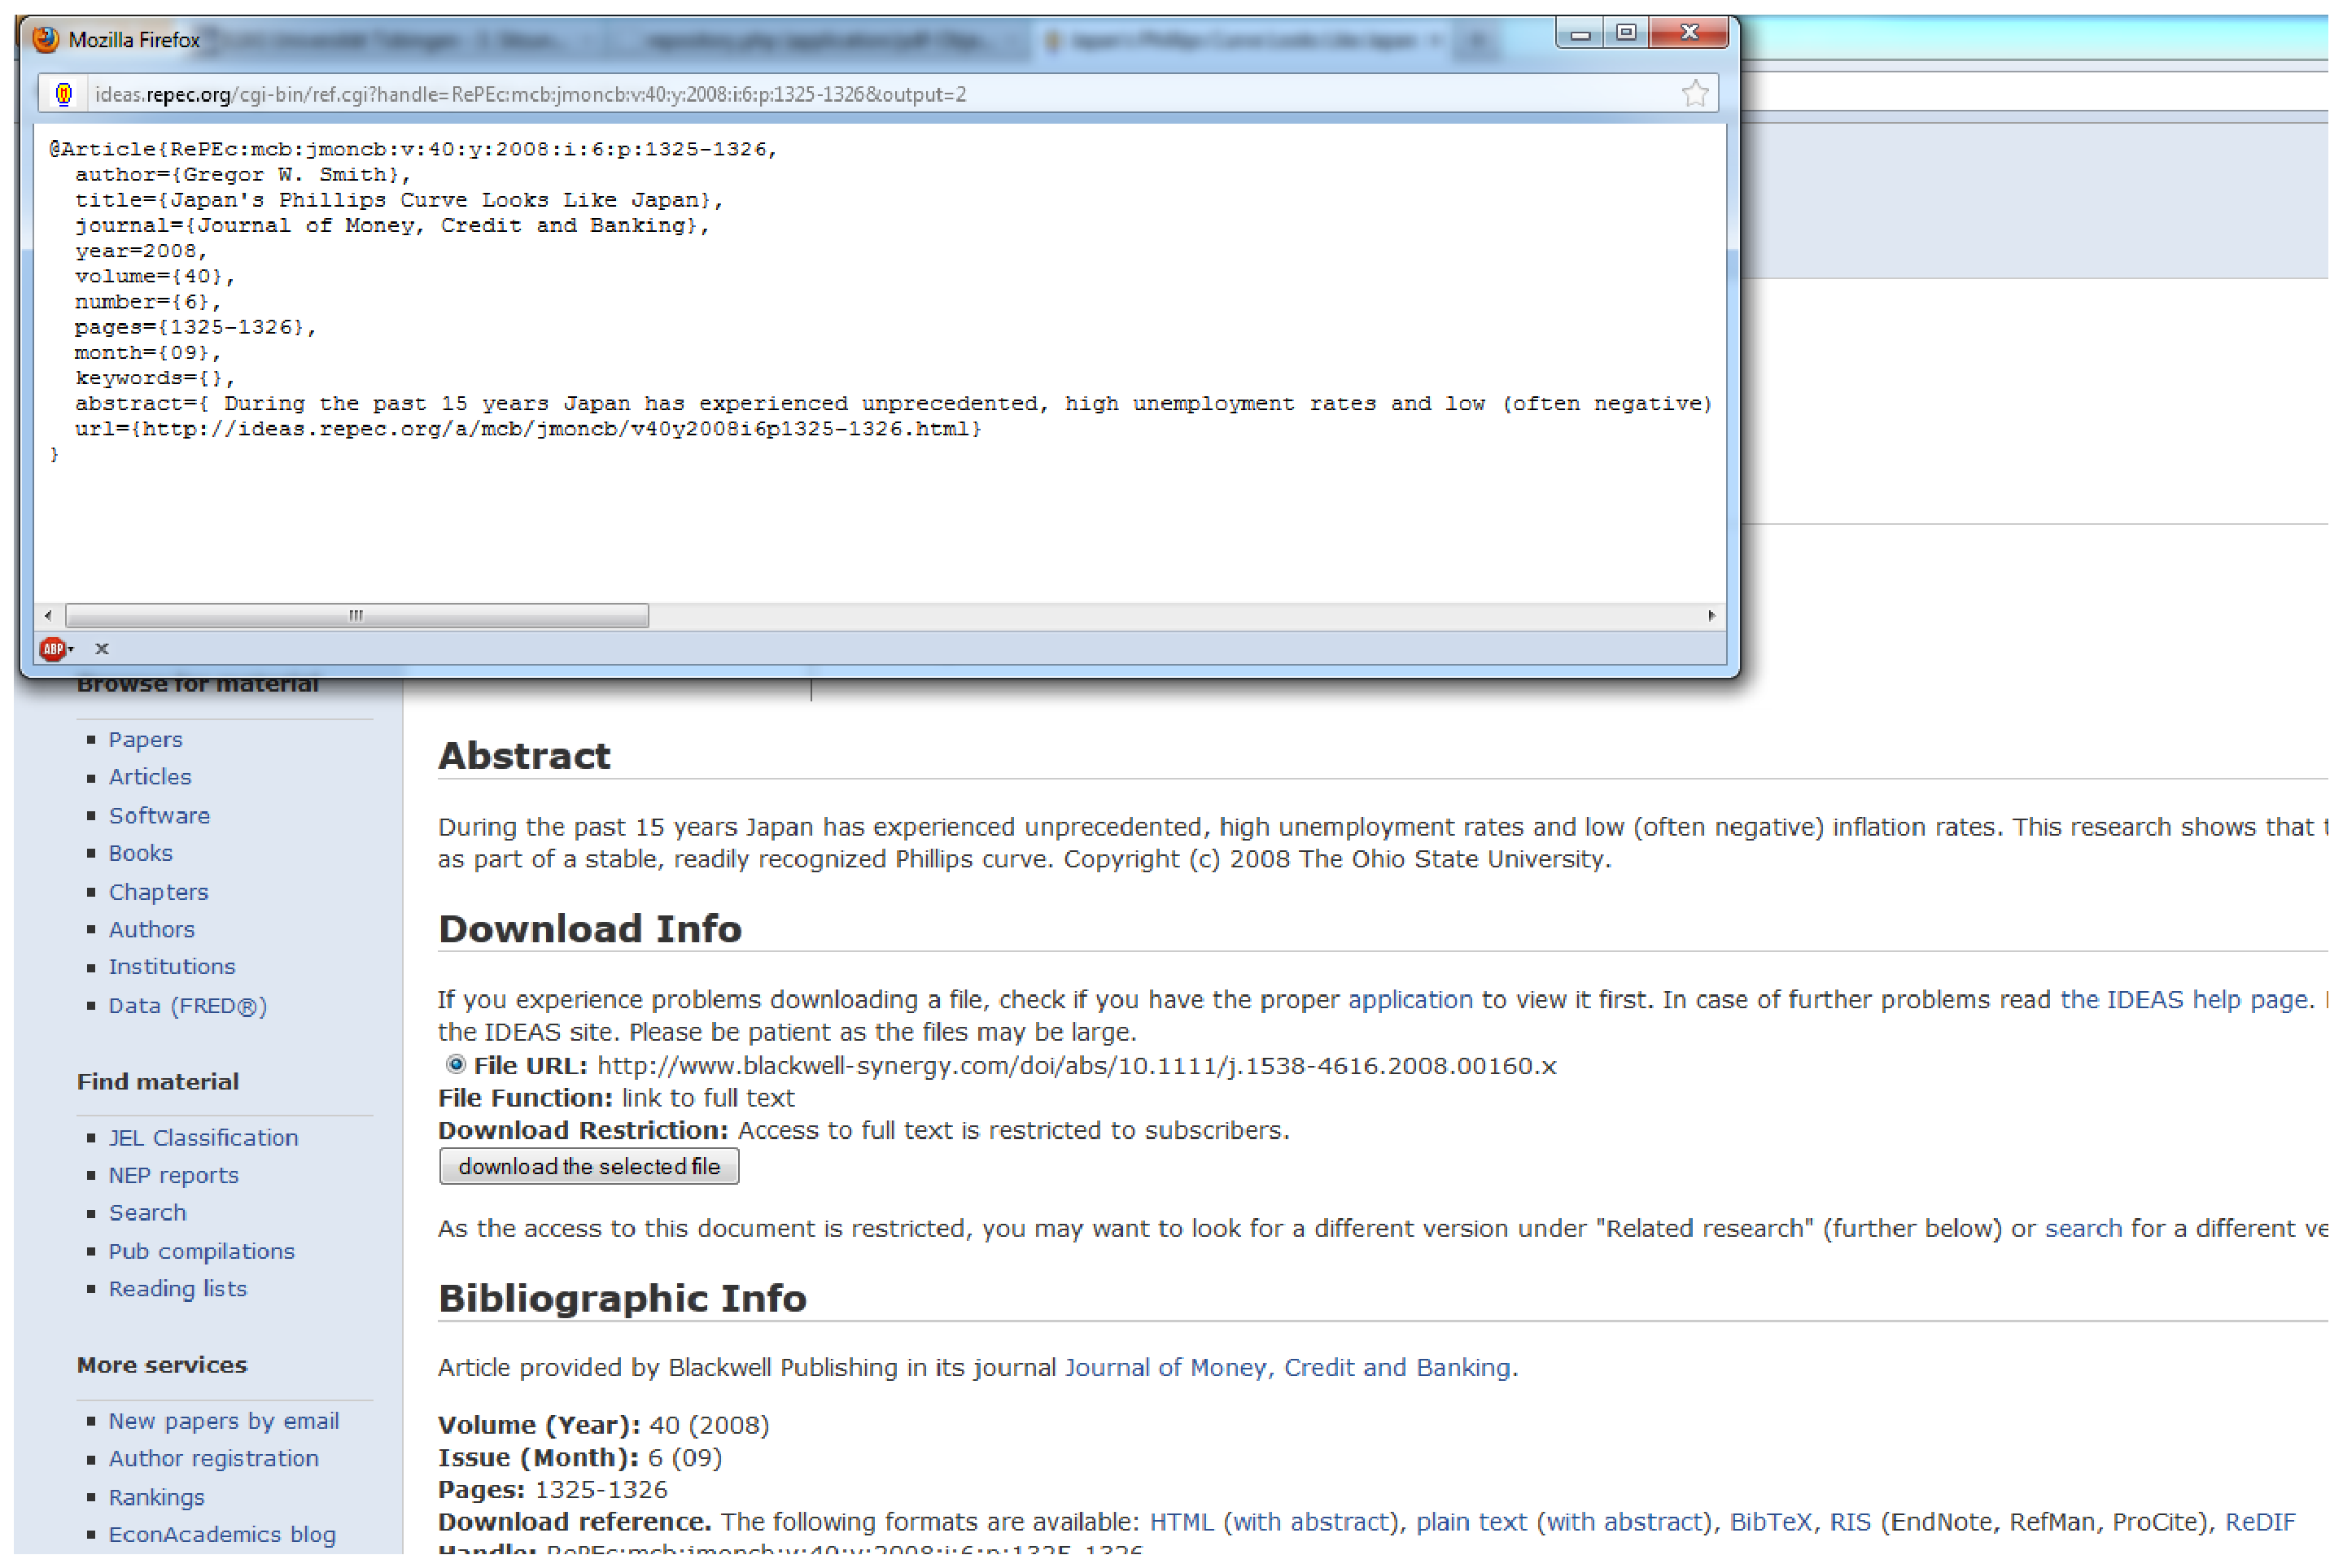
\includegraphics[width=\ScaleIfNeeded]{Ideasbibtex}
%\caption[Extracting References from Bibtex]{Copy the text from the window into the memory}\label{fig:Ideas2}
%\end{figure}
%%
%\begin{figure}[htbp!]
%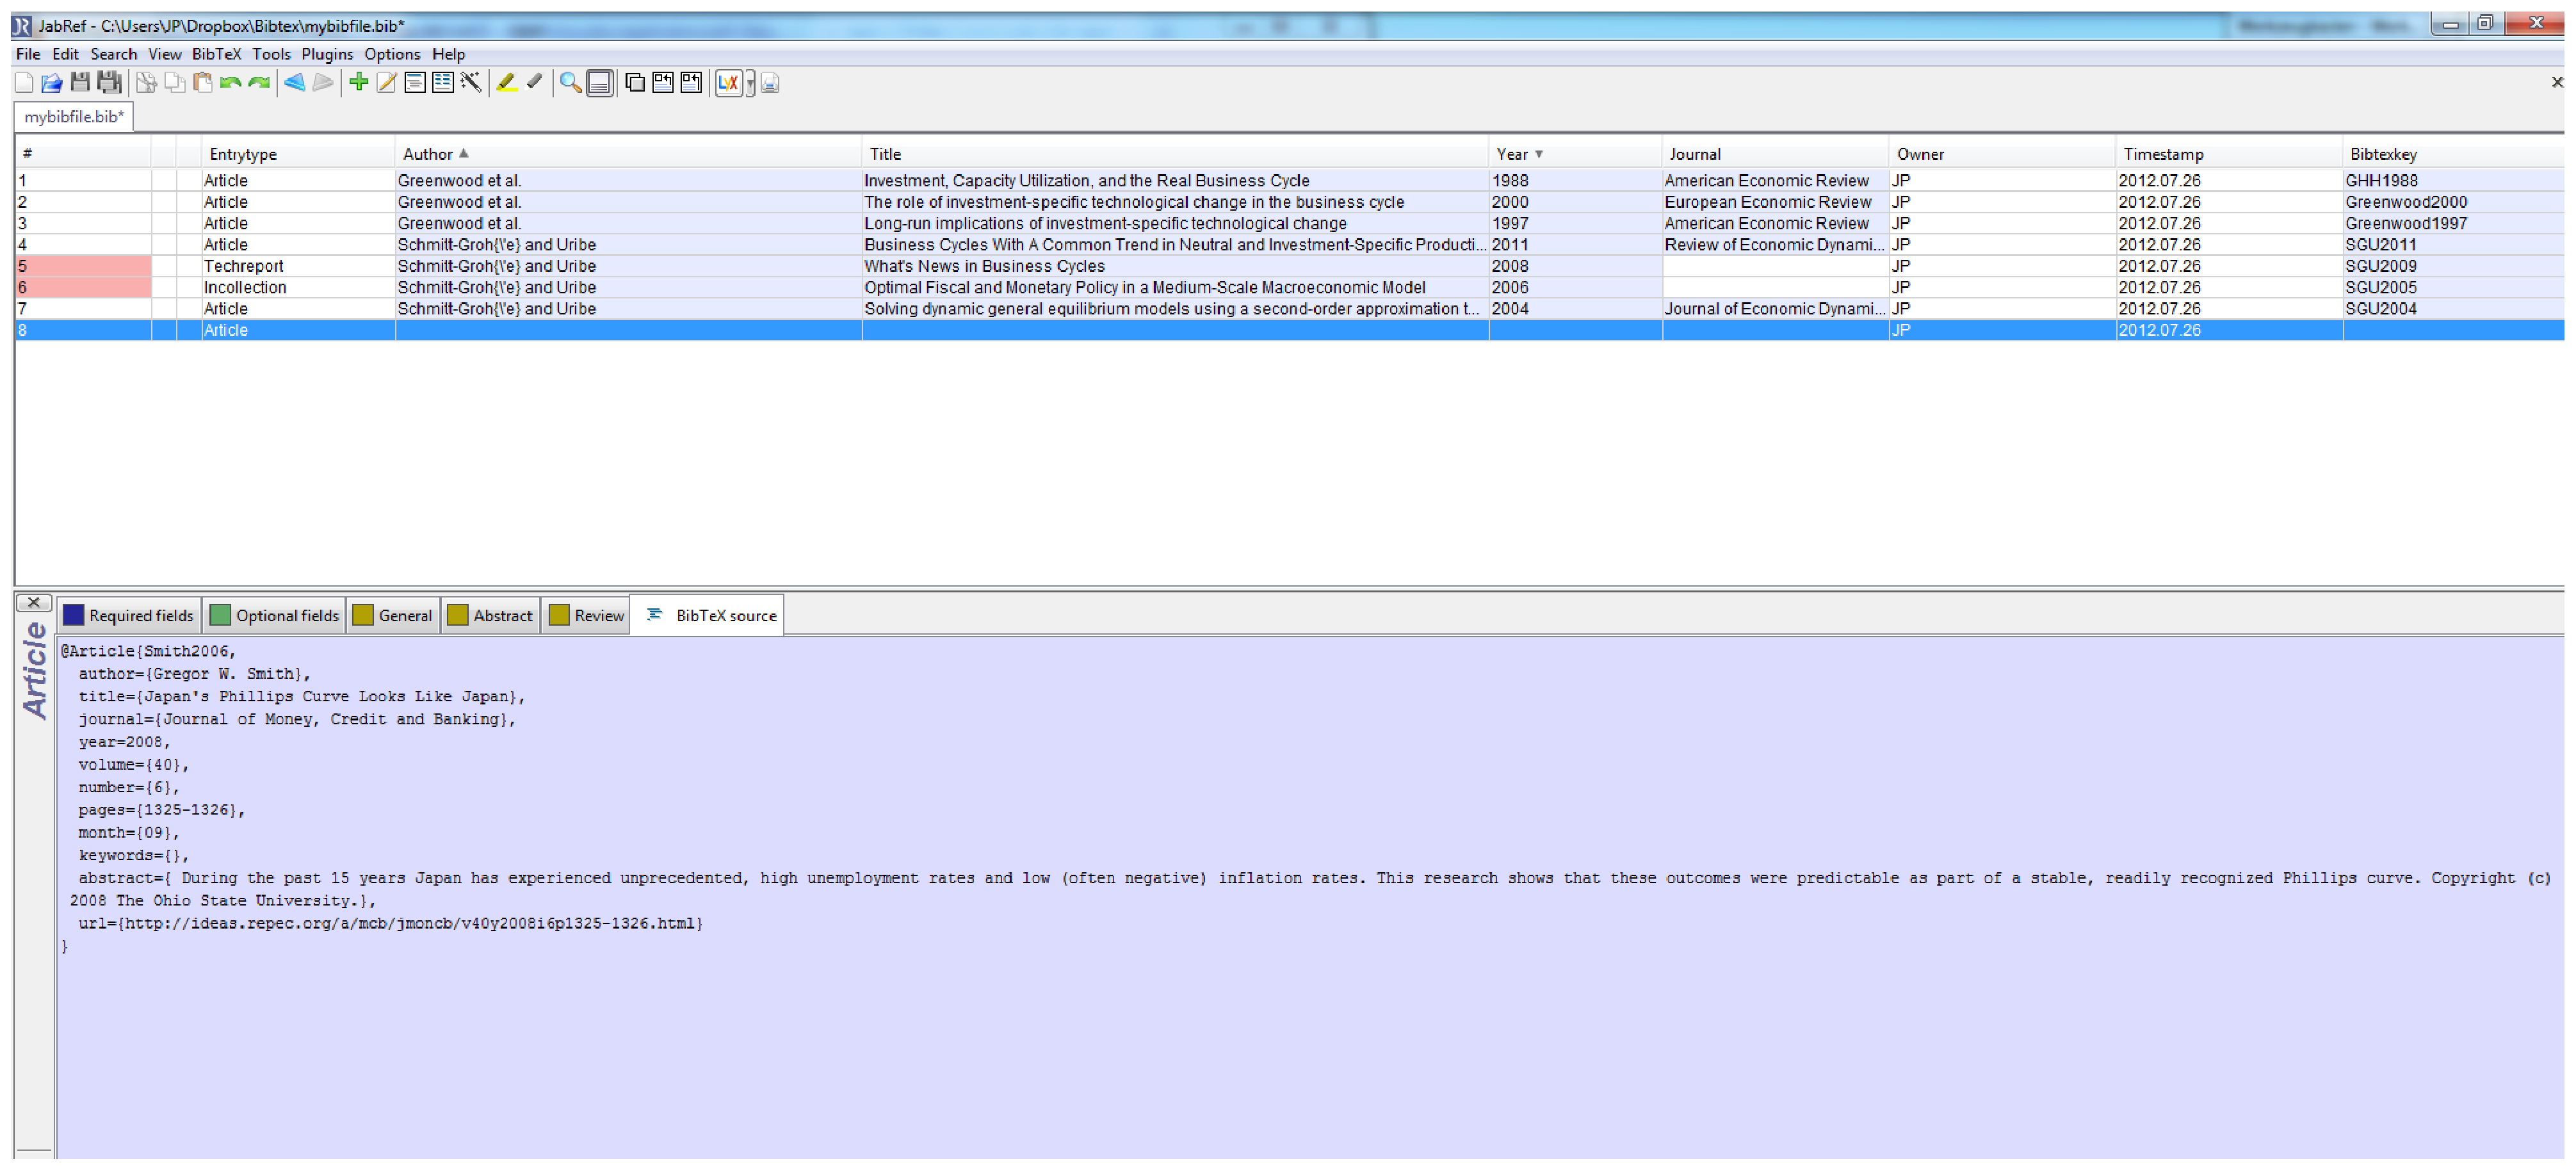
\includegraphics[width=\ScaleIfNeeded]{JabrefAdd}
%\caption[Using JabRef]{Klick on the Add-Button (green plus) and paste the copied text to \emph{Bibtex Source}. Do not forget to change the Bibtex-key (the first entry). Here I chose the key \texttt{Smith2006}}\label{fig:jabref}
%\end{figure}
%
%Please use inline citations and not citations in footnotes.\interfootnotelinepenalty=5000\footnote{As you can see, footnotes are placed with the \texttt{\textbackslash footnote{}}-command. Sometimes footnotes can become quite long. In this case, \LaTeX\ automatically distributes the footnote over more than one page. Sometimes this automatic setting does not perform the way it should. You can change the behavior by setting \texttt{\textbackslash interfootnotelinepenalty=x}, where $x$ is an integer from $0$ to $10{,}000$, with 100 being the default. When set to $10{,}000$ \LaTeX\ will not split the footnote. The option \texttt{\textbackslash interfootnotelinepenalty=x} can be both set in the preamble to affect all footnotes or in the text immediately before a footnote. In the latter case, it needs to be set back to its default if you want the command to only affect one footnote.} \interfootnotelinepenalty=100  The \texttt{natbib}-compatibility specified in the preamble provides several cite commands.\footnote{For the original Bib\LaTeX-commands that allow for many more options, see \url{http://mirror.ctan.org/macros/latex/contrib/biblatex/doc/biblatex.pdf}.} The command \texttt{\textbackslash citet\{Smith2006\}}, where \textit{Smith2006} is the Bibtex-Key defined in JabRef, cites the reference with the name: \citet{Smith2006}. The command \texttt{\textbackslash citep\{Smith2006\}} cites the reference in parentheses: \citep{Smith2006}. The command \verb|\citep[Prefix][Suffix]\{Smith2006\}| allows for Prefixes and Suffixes in the parentheses: \citep[see e.g.][pp. 1-4]{Smith2006}. More information can be found at \url{ftp://ftp.tex.ac.uk/tex-archive/macros/latex/contrib/natbib/natnotes.pdf}.\\
%
%Bib\LaTeX automatically shortens multiple citations with the same authors, e.g.\ \citep{SGU2004JET,SGU2004,SGU2009,SGU2011} and provides correct referencing with a,b,etc. Moreover, it takes care of different bibliography requirements of articles like \citet{SGU2004} and books like e.g.\ \citet{SGU2005}.\\
%The style of the bibliography is controlled using the \verb|bibstyle|-option. The current document uses the JME-style file.\\
%
%For electronic sources like blog-posts \citep[e.g.\ ][]{Krugman2012}, you should use the \texttt{electronic}-entrytype in JabRef. Unfortunately, you must manually add the \texttt{urldate}-field to the Bib\TeX-source as shown in Figure \ref{fig:jabref_urldate} in order to print out the access date. The correct field format is YYYY-MM-DD.
%
%\begin{figure}[htbp!]
%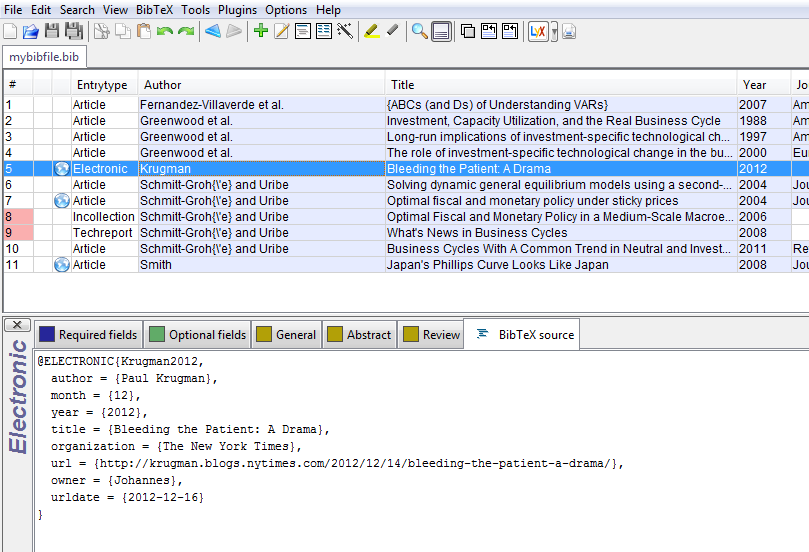
\includegraphics[width=\ScaleIfNeeded]{urldate}
%\caption[Adding electronic sources]{For electronic sources, you must manually enter the \texttt{urldate}-field in the Bib\TeX source.}\label{fig:jabref_urldate}
%\end{figure}
%
%
%\section{List of Symbols and Abbreviations}
%A List of Symbols and a List of Abbreviations as displayed at the beginning of this document can be created using the \texttt{glossaries} package.\footnote{For more information, see the beginner's guide at \url{http://mirror.ctan.org/macros/latex/contrib/glossaries/glossariesbegin.pdf} and the documentation at \url{http://mirror.ctan.org/macros/latex/contrib/glossaries/glossaries.pdf}.} In case you are using TeXnicCenter, you may have to manually add makeindex to the profile.\footnote{See \url{http://brianhoffmann.de/journal/thesis/2011-08-01/latex-glossaries-with-texniccenter/} or \url{https://tex.stackexchange.com/questions/153323/acronyms-glossaries-not-being-output-in-the-pdf/}.}
%
%\subsection{The \texttt{glossaries} package in the preamble}
%The \texttt{glossaries} package is one of the few packages that must be loaded after the \texttt{hyperref}-package. In the current document, I use the standard glossary to list acronyms. In addition to the default glossary, I have defined a second glossary for the List of Symbols, labeled \texttt{symbolslist}, using the command\\
%\verb|\newglossary[slg]{symbolslist}{syi}{syg}{List of Symbols}|.\\
%
%After defining the glossaries, you must put \verb|\makeglossaries| to allow for sorting of the glossary entries.\\
%
%To print the List of Abbreviations, put\\
%\verb|\printglossary[type=\acronymtype,style=long]|.\footnote{Of course, the style can be changed.}\\
%To print the List of Symbols, put\\
%\verb|\printglossary[type=symbolslist,style=long,title=List of Symbols]|.
%
%\subsection{Defining the list entries and referencing them}
%The entries for the glossaries can either be defined in the preamble or in the main text. For example, the command
%\verb|\newglossaryentry{symb:pi}{name={\ensuremath{\pi}}...|, used in the preamble of this document, defines an entry for the glossary \texttt{symbolslist}. However, the symbol \gls{symb:pi} will not appear in the List of Symbols unless you tell \LaTeX\ that you have used it. Usually, you do this by referencing it using the \verb|\gls{}|-command. For example, \verb|\gls{symb:pi}| prints \gls{symb:pi}. This command can also be used inside of equations like this one
%
%\begin{equation}
%  \gls{symb:e}^{\gls{symb:i}\gls{symb:pi}}-1=0
%\end{equation}
%
%\newacronym{acro:DSGE}{DSGE}{Dynamic Stochastic General Equilibrium} %define new acronym inside of the main document
%
%You can also define symbols or acronyms in the main matter, for example putting \verb|\newacronym{acro:DSGE}{DSGE}{Dynamic Stochastic General Equilibrium}| at the beginning or end of a paragraph where you use the symbol/acronym the first time. Subsequently in the text, you can refer to the acronym using the command \verb|\gls{}|, e.g.\ \verb|\gls{acro:DSGE}|. The first time you use it, \LaTeX\ automatically prints the long version followed by the abbreviation. The second time, only the acronym is printed. For example, \gls{acro:DSGE} will from now on be abbreviated as \gls{acro:DSGE}. Moreover, all symbols/abbreviations referenced with \verb|\gls{}| (or its derived commands) are automatically added to the list of symbols/abbreviations.\\
%\textbf{For glossaries to be updated correctly, you usually have to run \LaTeX\ (at least) twice.}\\
%
%If you are not going for the full capabilities of glossaries, you can also just define the symbol or acronym you are using in the preamble and add it to the respective list by putting \verb|\glsadd{}| after the definition as I did with the \verb|\glsadd{OLS}|. In this case, the symbol/acronym will appear in the List of Symbols/Abbrevations even if you did not reference it with \verb|\gls{}|. Hence, this is an quick and dirty way to create such a list. However, this procedure is not advised as you now have to make sure manually that only abbreviations/symbols used at least once in the text appear in the list.
%

%
%\section{Further Information}
%
%\begin{itemize}
%    \item Almost every imaginable \LaTeX-question has been asked before. Just google or search the FAQ at \url{http://www.tex.ac.uk/cgi-bin/texfaq2html?introduction=yes}
%    \item There are deadly \LaTeX\ sins you should never commit, see \url{http://queen.elektro.uni-miskolc.hu/~gati/references/latex/latex/l2tabuen.pdf}.
%    \item Helpful resources can be found at \url{http://en.wikibooks.org/wiki/LaTeX/}.
%    \item For presentations use \LaTeX\ Beamer, see \url{ftp://ftp.fu-berlin.de/tex/CTAN/macros/latex/contrib/beamer/doc/beameruserguide.pdf}.
%\end{itemize}

%_________________ End of Main Matter_________________%

\clearpage

%_________________ Reference Section _______________%

\phantomsection                                   % allows for correct link to Table of Contents
\addcontentsline{toc}{section}{References}        % Adds the line "References" to Table of contents
\onehalfspacing


%\printbibliography % print the bibliography using BibLaTex


%% alternative using BibTeX
%\bibliographystyle{econometrica}                  % sets the style for the Bibliography
%\bibliography{mybibfile}                         % Uses the Bibtex-file mybibfile.bib


\clearpage
%_________________ Space for Supplementary Material _______________%
\appendix
\numberwithin{equation}{section} %restarts equation numbering with 1 and adds the appendix in front
\numberwithin{table}{section} %same for Tables
\numberwithin{figure}{section} %and for Figures

%\section{Appendix 1}
%
%Some Information relegated to the appendix.
%\begin{equation}
%    MV=PQ
%\end{equation}
%
%\pagebreak
%
%\section{Supplementary Tables}
%



%\begin{table}[h!] % h! places the float at this place, use t for top or b for bottom
%\caption{Title of the table}
%\label{tab:SuppTable1}
%\centering
% \begin{tabular}{lcr}
%   Another & small & table\\
%\toprule
%   left aligned & centered & right aligned \\
%   \multicolumn{2}{c}{Text over two columns} & third column \\
%\bottomrule
%\end{tabular}
%\caption*{\footnotesize{\emph{Notes:} Add the description here}}
%\end{table}

\clearpage


\end{document}
